\documentclass[a4paper]{exam}

\usepackage{hyperref}
\usepackage{graphicx}
\usepackage{siunitx}
\usepackage{multicol}

\begin{document}
\begin{center}
  \huge{\textbf{Level 2 Physics Assignment}}\\
  \huge{\textbf{The Stanford Linear Accelerator}}
\end{center}

\section{Background}
\begin{center}
  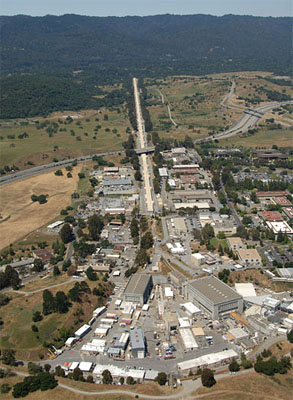
\includegraphics[height=0.25\textheight]{slac1}
  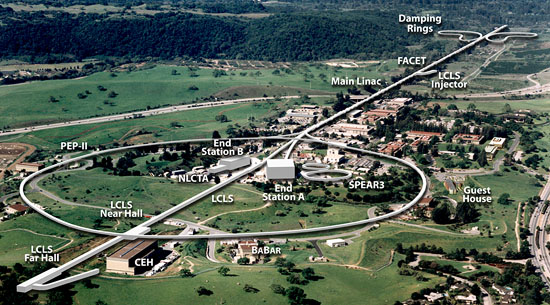
\includegraphics[height=0.25\textheight]{slac2}
\end{center}
The Stanford two-mile accelerator, the longest in the world, accelerates electrons to the very high energy needed in the study of subatomic particles and forces. Experiments performed here have shown that the proton, one of the building blocks of the atom, is in turn composed of smaller particles now called quarks. Other research here has uncovered new families of particles and demonstrated subtle effects of the weak nuclear force. This research requires the utmost precision in the large and unique electromechanical devices and systems that accelerate, define, deliver, and store the beams of particles and in the detectors that analyze the results of the particle of interactions.

{\scriptsize\textit{From \url{https://www.asme.org/about-asme/who-we-are/engineering-history/landmarks/92-stanford-linear-accelerator-center}.}}

\section{Useful Data and Notes}
\begin{multicols}{3}
\begin{itemize}
  \item Mass of an electron:\\ $ m_e = \SI{9.11e-31}{\kilo\gram} $
  \item Charge on a proton:\\ $ e = \SI{1.60e-19}{\coulomb} $
  \item Speed of light in a vacuum: $ c = \SI{3.00e8}{\metre\per\second} $
  \item $ \SI{1}{\electronvolt} \equiv \SI{1.60e-19}{\joule} $
\end{itemize}

\textit{Important note:} A positron is a particle with the same mass as the electron but a positive charge (of the same magnitude) --- they are
a \textit{matter/antimatter pair}.

\begin{itemize}
  \item $ a = \frac{\Delta v}{\Delta t} $
  \item $ v_f = v_i + at $
  \item $ v_f^2 = v_i^2 + 2ad $
  \item $ F = ma $
  \item $ a_c = \frac{v^2}{r} $
  \item $ C = 2\pi r $
  \item $ F = q(\vec E + v \times \vec B) $\\ (Lorentz force equation)
  \item $ J = \Delta p = F \Delta t $
\end{itemize}
\end{multicols}

\section{Questions}
\begin{questions}
  \question The linear accelerator \SI{3.2}{\kilo\metre} long, and is capable of accelerating electrons and positrons up to \SI{50}{\giga\electronvolt}.
    \begin{parts}
      \part Given that the particles are accelerated from rest to their maximum energy, what is the overall change in kinetic energy
            of an electron due to the accelerator (in joules)?
      \part What is the final velocity of an electron? We must take into account relativity since the speed is so high: if the velocity of a
            particle is $ u $ then the kinetic energy $ E_K $ is given by
            \begin{displaymath}
              E_K = \frac{mc^2}{\sqrt{1 - \frac{u^2}{c^2}}} - mc^2.
            \end{displaymath}
      \part The accelerator accelerates particles uniformly (i.e. the acceleration is constant). How long does it take for an electron
            to travel from the start to the end of the accelerator?
      \part Calculate the impulse exerted on an electron by the acceleration (hint: impulse is just the change in momentum). Hence find
            the force exerted by the accelerator on the particle at each instant.
    \end{parts}
  \question After being accelerated to their final velocity, the protons and positrons are injected into a circular ring of circumference
            \SI{2.2}{\kilo\metre} (labelled as PIP-II in the diagram above).
    \begin{parts}
      \part What is the radius of each ring, in metres?
      \part What type of force is acting on the protons and particles in order to keep them confined to the circular ring? Given that their
            speed around the ring is constant, in which direction is the force acting on the particles?
      \part What is the magnitude of this force?
      \part The force whose magnitude you have calculated is actually due to a constant magnetic field $ \vec B $. Calculate the strength
            of this field.
      \part The magnetic field of the earth at the surface is around 65 microteslas. Compare this with your calculated magnetic field and say something intelligent.
      \part The same magnets are used to circulate both electrons and positrons around the holding ring. The electrons travel clockwise around the ring
            when looking down from above.
        \begin{subparts}
          \subpart In which direction around the ring do the positrons travel? Why?
          \subpart In which direction does the the vector $ \vec B $ point?
        \end{subparts}
    \end{parts}
  \question The purpose of the entire setup is to collide the electrons and positrons, which annihilate. At high enough energies, it
            is possible to produce W and Z bosons; however, more often than not the result is a pair of photons:
            \begin{displaymath}
              e^+ + e^- = \gamma + \gamma.
            \end{displaymath}
    \begin{parts}
      \part The overall kinetic energies of the particles do not change while they are in the ring. When they collide and annihilate, how much energy
            is available to create new particles?
      \part In a certain collision between an electron and a positron (both at maximum energy), two photons with identical energy are formed.
            The Plank-Einsten relation states that the energy of a photon is proportional to its frequency with a proportionality constant
            $ h = \SI{6.63e-34}{\joule\second} $ (Plank's constant):
            \begin{displaymath}
              E = hf
            \end{displaymath}
            What frequency of light is produced in the collision?
      \part Suppose that all the energy of a single photon of this light is transferred to the kinetic energy a car of mass \SI{1000}{\kilo\gram}. What would the
            speed of the car be (assuming no net force on the car)? Based on this, do you think that standing in front of the gamma rays would be
            a good idea? Explain.
%       \clearpage
      \part The gamma rays (light rays) produced are reflected and focused into an optical fibre made of lead glass ($ n = 1.8 $) surrounded by air.
        \begin{subparts}
          \subpart Name the phenomenon which allows the light to remain inside the fibre rather than refracting out, and give
                   the two conditions necessary for it to occur.
          \subpart For what angles of incidence will the light remain within the fibre?
        \end{subparts}
    \end{parts}
  \question Some of the light is directed to fall on a photo-voltaic cell, which is connected to two resistors in parallel.
    \begin{parts}
      \part The power on the cell happens to be \SI{200}{\watt}, and a current of \SI{40}{\ampere} is produced. What is the voltage across
            the cell?
      \part The magnitude of one of the resistors is \SI{2}{\ohm}. What is the magnitude of the other, and how much power does it dissipate? How long
            would it need to run before enough energy is generated to accelerate a single positron to full speed in the linear accelerator?
    \end{parts}
\end{questions}
\end{document}
